% =============================================================================
% PART B - MODULES 32 & 42: PROPOSAL MANAGEMENT & AI RECOMMENDATION
% (UC-34.01 - UC-34.09, UC-44.01)
% In Charge: Tran Phat Tai (CE181632)
% =============================================================================

\newpage
\subsection{Modules 32 \& 42: Proposal Management \& AI Job--Freelancer Recommendation}

The Proposal Management module orchestrates competitive bidding between identity-verified Freelancers and Clients---covering draft authoring, submission with budget/deadline safeguards, editing, withdrawal, client pipeline review, rejection, and one-click contract creation upon hiring. Complementing this flow, the AI Recommendation engine ranks open jobs for Freelancers (\texttt{cv2jd}) and qualified candidates for Clients (\texttt{jd2cv}) using hybrid semantic, skill, experience, and budget scoring.

% -----------------------------------------------------------------------------
\subsubsection{M32.01 -- View My Proposals List (UC-34.01)}

\begin{itemize}[leftmargin=1.5em,itemsep=2pt]
  \item \textbf{Screen Name \& Route Path:} My Proposals -- \texttt{/freelancer/\allowbreak{}proposals}.
  \item \textbf{Target Actor:} Freelancer (Identity Verified).
  \item \Needspace{6\baselineskip}\textbf{Before You Begin:} Sign in as a Freelancer with approved eKYC identity verification.
\end{itemize}
\begin{figure}[H]\centering
  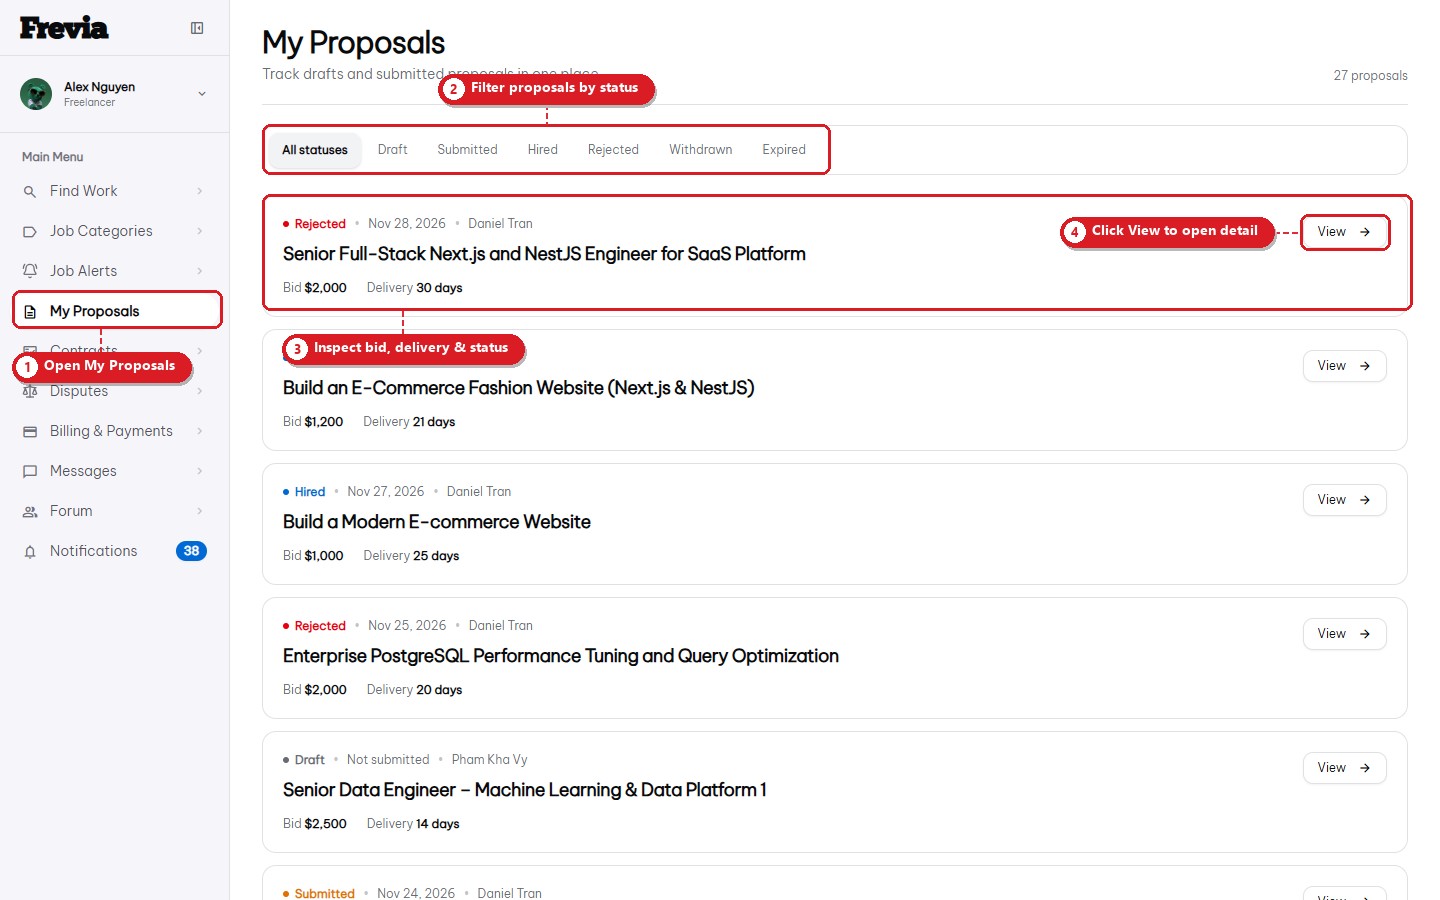
\includegraphics[width=0.90\textwidth]{images/jobs_proposals/m32_01_view_my_proposals_guide.png}
  \caption{Freelancer My Proposals dashboard with lifecycle status filter tabs and summary cards}
  \label{fig:m32_01_view_my_proposals}
\end{figure}
\Needspace{6\baselineskip}\paragraph{Step-by-Step User Guide:}
\begin{enumerate}[leftmargin=1.8em,itemsep=3pt]
  \item \rbadge{1} \textbf{Open My Proposals:} Select \textbf{My Proposals} from the left navigation sidebar.
  \item \rbadge{2} \textbf{Filter by Status Tab:} Switch between \textbf{All statuses}, \textbf{Draft}, \textbf{Submitted}, \textbf{Hired}, \textbf{Rejected}, \textbf{Withdrawn}, and \textbf{Expired}.
  \item \rbadge{3} \textbf{Review Proposal Cards:} Inspect each card's status indicator, submission date, Client name, job title, bid amount, and delivery days.
  \item \rbadge{4} \textbf{Open Full Detail:} Click \textbf{View} on the right side of any proposal card to view, edit, submit, or withdraw it.
\end{enumerate}
\Needspace{6\baselineskip}\paragraph{After You Submit (Result \& Troubleshooting):}
\begin{itemize}[leftmargin=1.5em,itemsep=2pt]
  \item \textbf{What Happens Next:} Overdue pending proposals past their job expiry are expired automatically before the paginated list renders.
  \item \textbf{Troubleshooting \& Common Messages:} Unverified accounts receive HTTP 403 \textit{IdentityNotVerified} until eKYC verification is approved.
\end{itemize}

% -----------------------------------------------------------------------------
\newpage
\subsubsection{M32.02 -- View My Proposal Details (UC-34.02)}

\begin{itemize}[leftmargin=1.5em,itemsep=2pt]
  \item \textbf{Screen Name \& Route Path:} My Proposal Detail -- \texttt{/freelancer/\allowbreak{}proposals/\allowbreak{}[id]}.
  \item \textbf{Target Actor:} Freelancer (Proposal Owner, Identity Verified).
  \item \Needspace{6\baselineskip}\textbf{Before You Begin:} Click \textbf{View} on any proposal from \texttt{/freelancer/proposals}.
\end{itemize}
\begin{figure}[H]\centering
  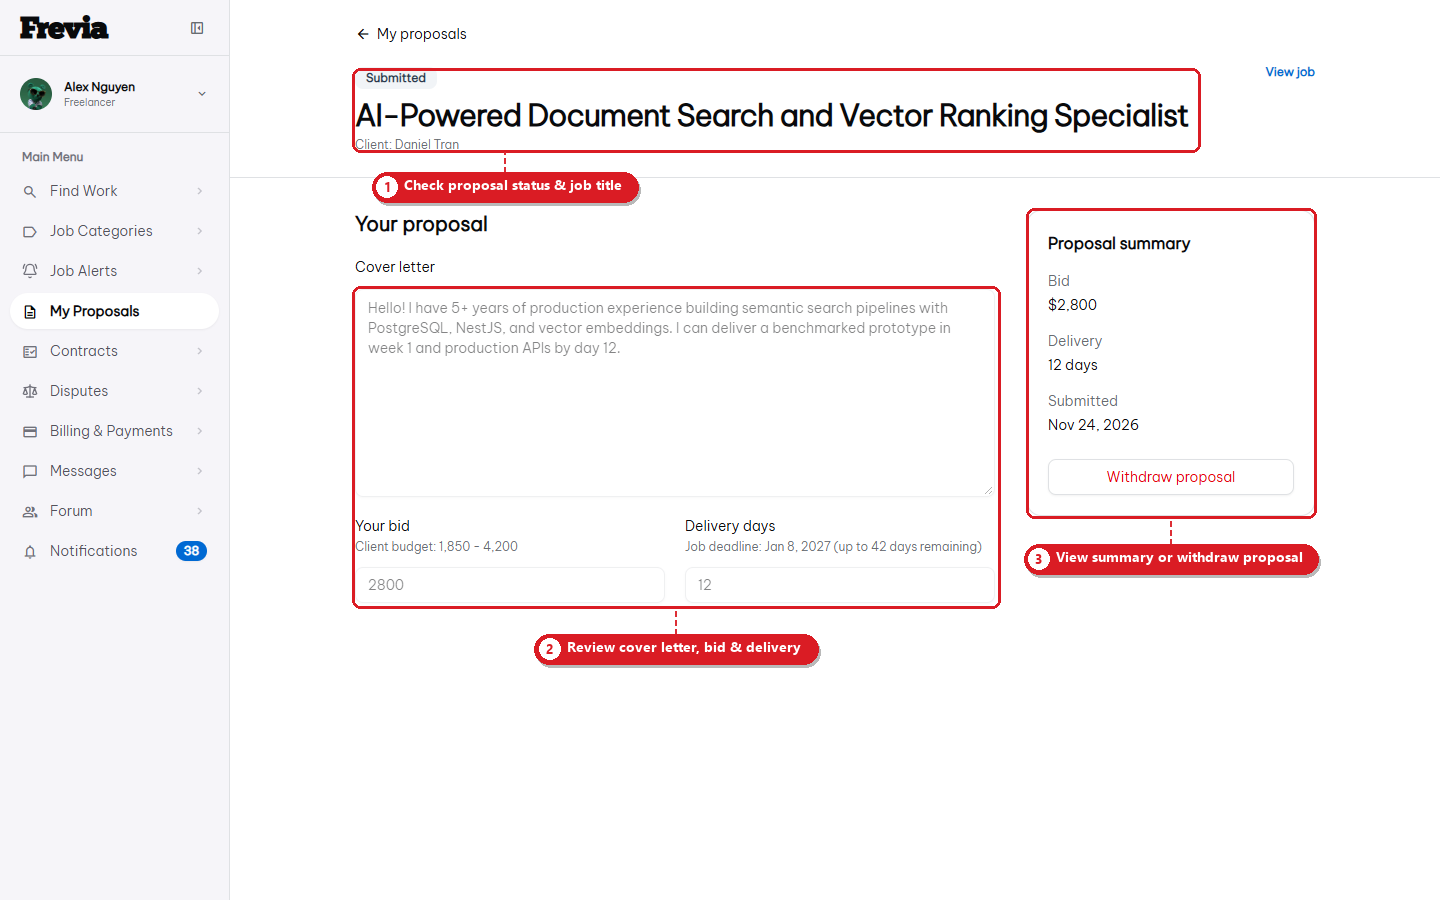
\includegraphics[width=0.90\textwidth]{images/jobs_proposals/m32_02_view_my_proposal_detail_guide.png}
  \caption{Freelancer Proposal Detail screen displaying status, cover letter, bid, and summary sidebar}
  \label{fig:m32_02_view_my_proposal_detail}
\end{figure}
\Needspace{6\baselineskip}\paragraph{Step-by-Step User Guide:}
\begin{enumerate}[leftmargin=1.8em,itemsep=3pt]
  \item \rbadge{1} \textbf{Check Status \& Target Job:} Review the current status pill (\textit{Submitted}, \textit{Draft}, \textit{Hired}, etc.), job title, and Client name (or click \textbf{View job} at top-right).
  \item \rbadge{2} \textbf{Review Cover Letter, Bid \& Delivery:} Inspect your submitted pitch, proposed USD bid against the Client's budget range, and delivery days.
  \item \rbadge{3} \textbf{Use Proposal Summary Panel:} Check key timestamps in \textbf{Proposal summary} or click \textbf{Withdraw proposal} if the proposal is still \texttt{SUBMITTED}.
\end{enumerate}
\Needspace{6\baselineskip}\paragraph{After You Submit (Result \& Troubleshooting):}
\begin{itemize}[leftmargin=1.5em,itemsep=2pt]
  \item \textbf{What Happens Next:} Full proposal terms and linked job metadata render cleanly; submitted proposals remain read-only until decided or withdrawn.
  \item \textbf{Troubleshooting \& Common Messages:} Accessing another Freelancer's proposal ID returns HTTP 403 \textit{Forbidden} or HTTP 404 \textit{ProposalNotFound}.
\end{itemize}

% -----------------------------------------------------------------------------
\newpage
\subsubsection{M32.03 -- Submit Proposal (UC-34.03)}

\begin{itemize}[leftmargin=1.5em,itemsep=2pt]
  \item \textbf{Screen Name \& Route Path:} Submit a Proposal Modal -- \texttt{/freelancer/\allowbreak{}jobs/\allowbreak{}[slug]}.
  \item \textbf{Target Actor:} Freelancer (Identity Verified).
  \item \Needspace{6\baselineskip}\textbf{Before You Begin:} Open an eligible \texttt{OPEN} job posting (not owned by you, before its expiry date, with no existing active proposal) and click \textbf{Apply now}.
\end{itemize}
\begin{figure}[H]\centering
  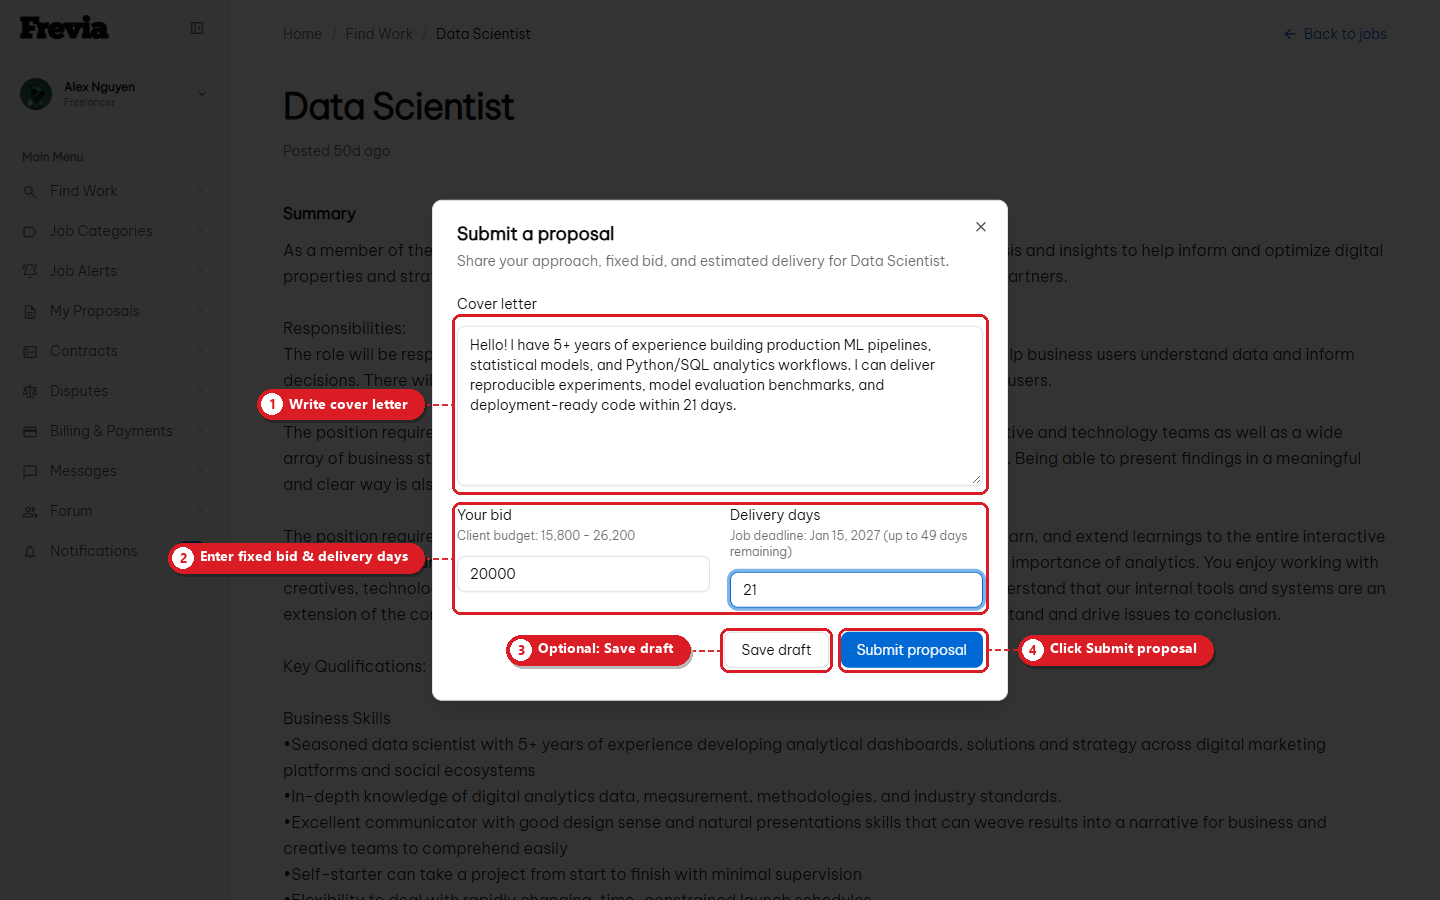
\includegraphics[width=0.90\textwidth]{images/jobs_proposals/m32_03_submit_proposal_guide.png}
  \caption{Submit a Proposal modal with cover letter composer, bid/delivery safeguards, and Save draft option}
  \label{fig:m32_03_submit_proposal}
\end{figure}
\Needspace{6\baselineskip}\paragraph{Step-by-Step User Guide:}
\begin{enumerate}[leftmargin=1.8em,itemsep=3pt]
  \item \rbadge{1} \textbf{Write Cover Letter:} Explain your relevant experience, technical approach, and planned deliverables in the \textit{Cover letter} textarea.
  \item \rbadge{2} \textbf{Enter Bid \& Delivery Days:} Input your fixed USD bid in \textit{Your bid} (referencing the displayed Client budget range) and estimated completion time in \textit{Delivery days} (within the remaining days until job deadline).
  \item \rbadge{3} \textbf{Save Draft (Optional):} Click \textbf{Save draft} if you want to store your proposal as a private \texttt{DRAFT} and refine it later.
  \item \rbadge{4} \textbf{Click Submit Proposal:} Click the blue \textbf{Submit proposal} button to send your application directly to the Client.
\end{enumerate}
\Needspace{6\baselineskip}\paragraph{After You Submit (Result \& Troubleshooting):}
\begin{itemize}[leftmargin=1.5em,itemsep=2pt]
  \item \textbf{What Happens Next:} The proposal is created with status \texttt{SUBMITTED} (or \texttt{DRAFT}) and appears in both your \textbf{My Proposals} list and the Client's job proposal pipeline.
  \item \textbf{Troubleshooting \& Common Messages:} Submitting without approved eKYC returns HTTP 403 \textit{IdentityNotVerified}; bids outside safeguard thresholds, delivery days exceeding the job deadline, or duplicate active proposals return HTTP 400/409 alerts.
\end{itemize}

% -----------------------------------------------------------------------------
\newpage
\subsubsection{M32.04 -- Update Draft Proposal (UC-34.04)}

\begin{itemize}[leftmargin=1.5em,itemsep=2pt]
  \item \textbf{Screen Name \& Route Path:} Edit Draft Proposal -- \texttt{/freelancer/\allowbreak{}proposals/\allowbreak{}[id]}.
  \item \textbf{Target Actor:} Freelancer (Proposal Owner, Identity Verified).
  \item \Needspace{6\baselineskip}\textbf{Before You Begin:} Open a proposal currently in \texttt{DRAFT} status from \textbf{My Proposals} $\rightarrow$ \textbf{Draft}.
\end{itemize}
\begin{figure}[H]\centering
  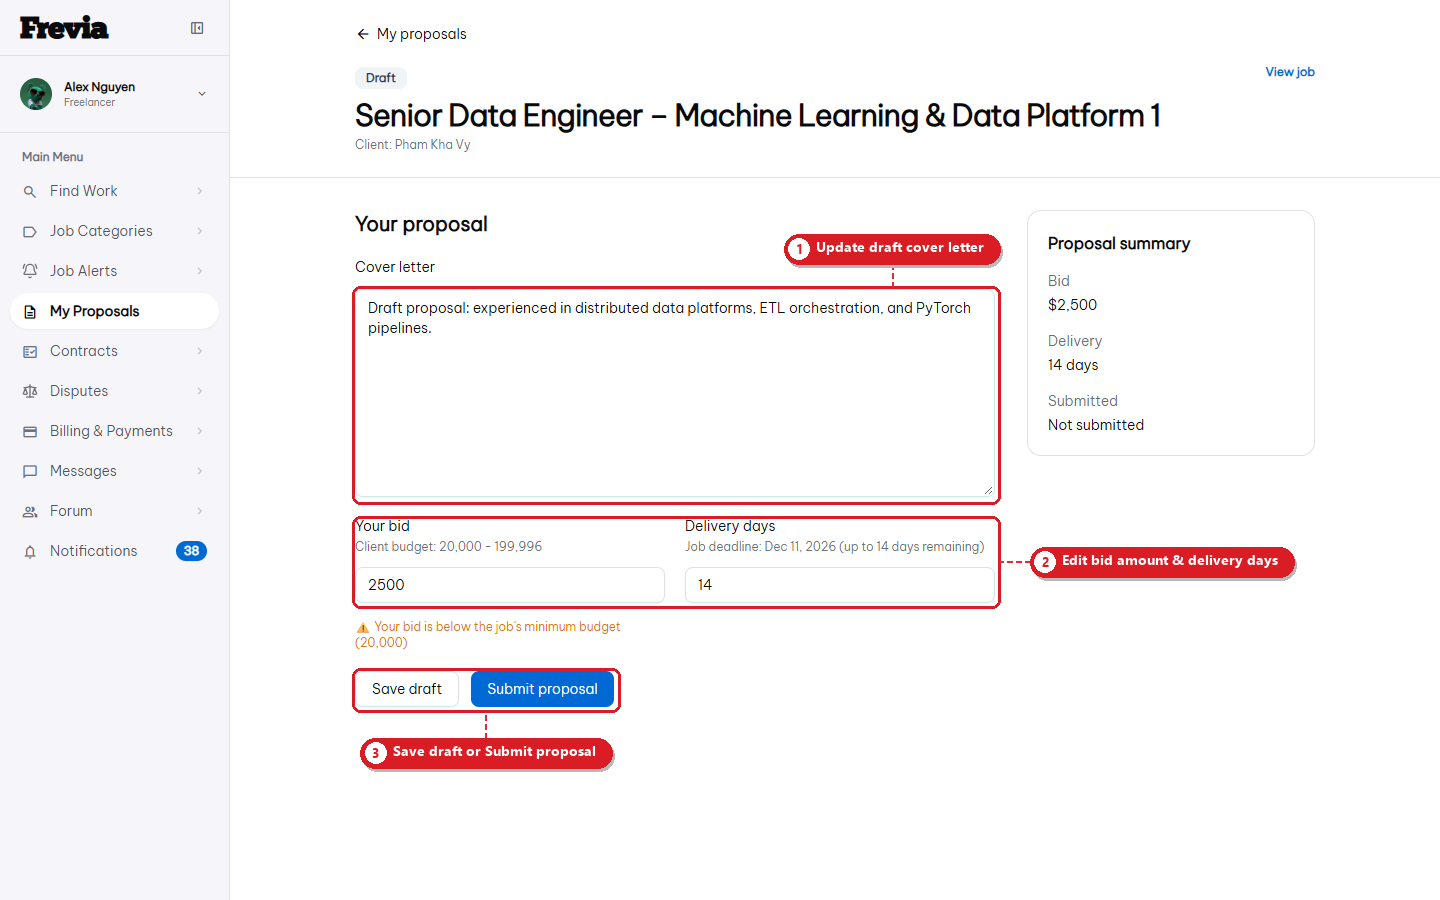
\includegraphics[width=0.90\textwidth]{images/jobs_proposals/m32_04_update_proposal_guide.png}
  \caption{Draft Proposal editor with budget safeguard notice, Save draft, and Submit proposal actions}
  \label{fig:m32_04_update_proposal}
\end{figure}
\Needspace{6\baselineskip}\paragraph{Step-by-Step User Guide:}
\begin{enumerate}[leftmargin=1.8em,itemsep=3pt]
  \item \rbadge{1} \textbf{Revise Cover Letter:} Edit your pitch and delivery outline directly in the \textit{Cover letter} editor.
  \item \rbadge{2} \textbf{Adjust Bid \& Delivery Days:} Update \textit{Your bid} and \textit{Delivery days}, addressing any amber safeguard notice (e.g., bid below the job's minimum budget).
  \item \rbadge{3} \textbf{Save Draft or Submit:} Click \textbf{Save draft} to store changes while staying in \texttt{DRAFT}, or click \textbf{Submit proposal} to finalize and send it to the Client.
\end{enumerate}
\Needspace{6\baselineskip}\paragraph{After You Submit (Result \& Troubleshooting):}
\begin{itemize}[leftmargin=1.5em,itemsep=2pt]
  \item \textbf{What Happens Next:} Draft edits save immediately; clicking \textbf{Submit proposal} transitions status to \texttt{SUBMITTED} and locks editing.
  \item \textbf{Troubleshooting \& Common Messages:} Proposals already \texttt{HIRED}, \texttt{REJECTED}, \texttt{WITHDRAWN}, or \texttt{EXPIRED} cannot be modified.
\end{itemize}

% -----------------------------------------------------------------------------
\newpage
\subsubsection{M32.05 -- Withdraw Proposal (UC-34.05)}

\begin{itemize}[leftmargin=1.5em,itemsep=2pt]
  \item \textbf{Screen Name \& Route Path:} Withdraw Proposal Confirmation Dialog -- \texttt{/freelancer/\allowbreak{}proposals/\allowbreak{}[id]}.
  \item \textbf{Target Actor:} Freelancer (Proposal Owner, Identity Verified).
  \item \Needspace{6\baselineskip}\textbf{Before You Begin:} Open an active \texttt{SUBMITTED} proposal and click \textbf{Withdraw proposal} in the right summary panel.
\end{itemize}
\begin{figure}[H]\centering
  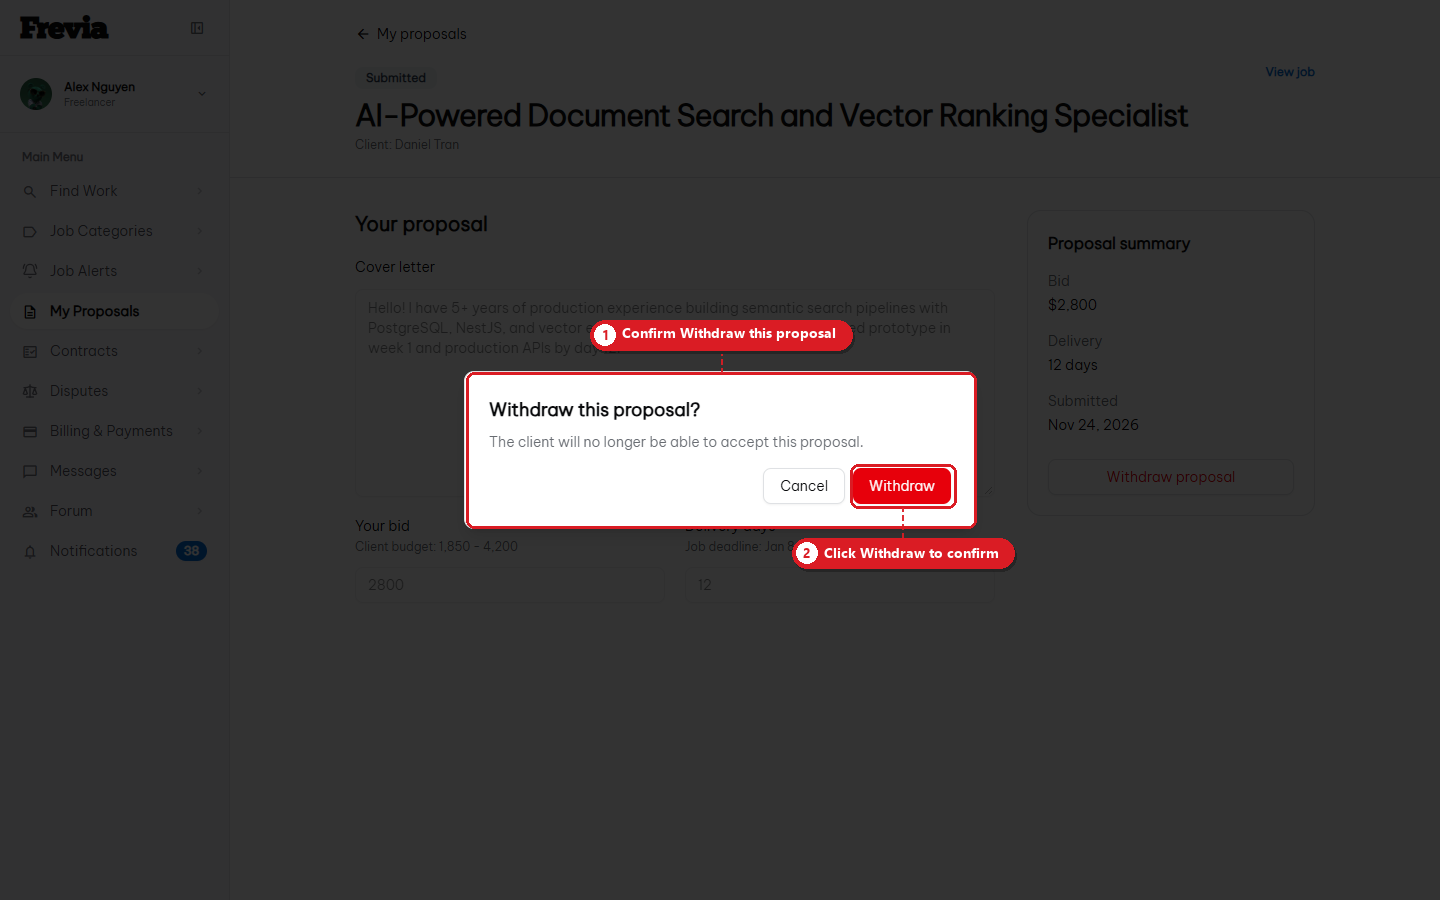
\includegraphics[width=0.90\textwidth]{images/jobs_proposals/m32_05_withdraw_proposal_guide.png}
  \caption{Withdraw proposal confirmation modal warning that the Client will no longer be able to accept}
  \label{fig:m32_05_withdraw_proposal}
\end{figure}
\Needspace{6\baselineskip}\paragraph{Step-by-Step User Guide:}
\begin{enumerate}[leftmargin=1.8em,itemsep=3pt]
  \item \rbadge{1} \textbf{Review Withdrawal Notice:} Confirm that withdrawing stops the Client from hiring this proposal.
  \item \rbadge{2} \textbf{Click Withdraw:} Click the red \textbf{Withdraw} button to finalize withdrawal (or \textbf{Cancel} to keep your proposal active).
\end{enumerate}
\Needspace{6\baselineskip}\paragraph{After You Submit (Result \& Troubleshooting):}
\begin{itemize}[leftmargin=1.5em,itemsep=2pt]
  \item \textbf{What Happens Next:} Proposal status updates to \texttt{WITHDRAWN} with a recorded \texttt{withdrawnAt} timestamp.
  \item \textbf{Troubleshooting \& Common Messages:} Proposals already accepted (\texttt{HIRED}) or decided (\texttt{REJECTED}) cannot be withdrawn and return HTTP 422 \textit{ProposalNotActionable}.
\end{itemize}

% -----------------------------------------------------------------------------
\newpage
\subsubsection{M32.06 -- Accept Proposal \& Hire Freelancer (UC-34.06)}

\begin{itemize}[leftmargin=1.5em,itemsep=2pt]
  \item \textbf{Screen Name \& Route Path:} Create Contract \& Hire Freelancer Drawer -- \texttt{/client/\allowbreak{}jobs/\allowbreak{}[jobId]/\allowbreak{}proposals}.
  \item \textbf{Target Actor:} Client (Job Owner, Identity Verified).
  \item \Needspace{6\baselineskip}\textbf{Before You Begin:} Open a job's proposal pipeline and click \textbf{Hire freelancer} on a \texttt{SUBMITTED} proposal (while the job has remaining hiring slots).
\end{itemize}
\begin{figure}[H]\centering
  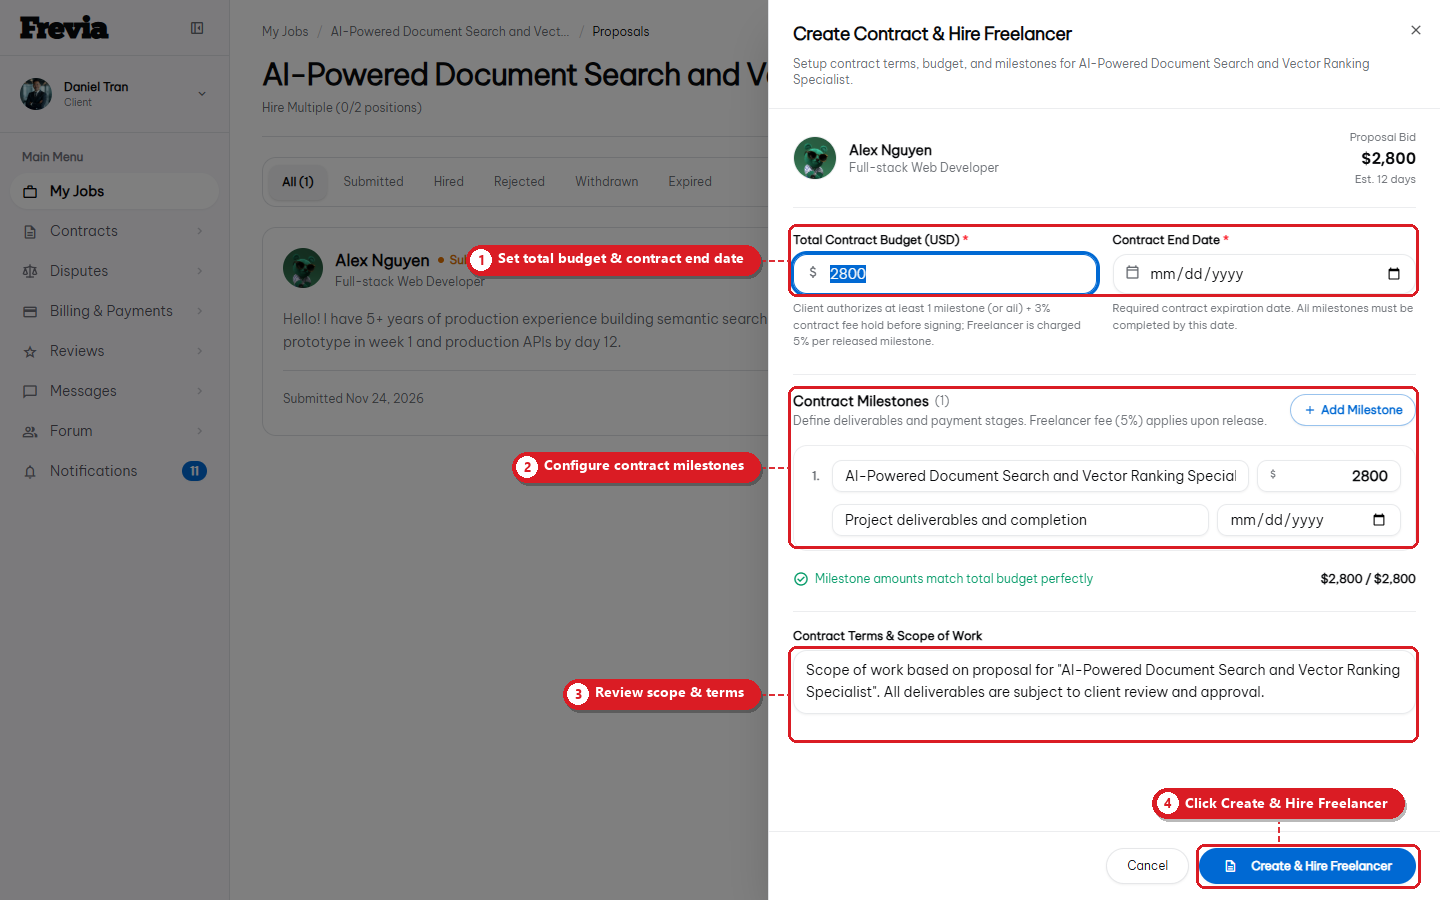
\includegraphics[width=0.90\textwidth]{images/jobs_proposals/m32_06_accept_proposal_guide.png}
  \caption{Create Contract \& Hire Freelancer slide-over drawer triggered when accepting a proposal}
  \label{fig:m32_06_accept_proposal}
\end{figure}
\Needspace{6\baselineskip}\paragraph{Step-by-Step User Guide:}
\begin{enumerate}[leftmargin=1.8em,itemsep=3pt]
  \item \rbadge{1} \textbf{Set Budget \& End Date:} Review the pre-filled \textit{Total Contract Budget (USD)} from the Freelancer's bid and choose a future \textit{Contract End Date}.
  \item \rbadge{2} \textbf{Configure Contract Milestones:} Verify the default milestone or click \textbf{+ Add Milestone} to split deliverables, ensuring milestone totals match the contract budget exactly.
  \item \rbadge{3} \textbf{Review Scope \& Terms:} Edit \textit{Contract Terms \& Scope of Work} to clarify acceptance criteria.
  \item \rbadge{4} \textbf{Click Create \& Hire Freelancer:} Click the blue \textbf{Create \& Hire Freelancer} button to accept the proposal and create the contract atomically.
\end{enumerate}
\Needspace{6\baselineskip}\paragraph{After You Submit (Result \& Troubleshooting):}
\begin{itemize}[leftmargin=1.5em,itemsep=2pt]
  \item \textbf{What Happens Next:} Within a database transaction, the proposal changes to \texttt{HIRED}, the contract and milestones are created, \texttt{positionsFilled} increments, an in-app notification is sent to the Freelancer, and if all slots are filled, remaining pending proposals are auto-cancelled.
  \item \textbf{Troubleshooting \& Common Messages:} Unverified Clients receive HTTP 403 \textit{IdentityNotVerified}; mismatched milestone sums or invalid dates return HTTP 422 validation errors.
\end{itemize}

% -----------------------------------------------------------------------------
\newpage
\subsubsection{M32.07 -- Reject Proposal (UC-34.07)}

\begin{itemize}[leftmargin=1.5em,itemsep=2pt]
  \item \textbf{Screen Name \& Route Path:} Reject Proposal Dialog -- \texttt{/client/\allowbreak{}jobs/\allowbreak{}[jobId]/\allowbreak{}proposals}.
  \item \textbf{Target Actor:} Client (Job Owner, Identity Verified).
  \item \Needspace{6\baselineskip}\textbf{Before You Begin:} Click \textbf{Reject} on a \texttt{SUBMITTED} proposal card or inside the proposal detail drawer.
\end{itemize}
\begin{figure}[H]\centering
  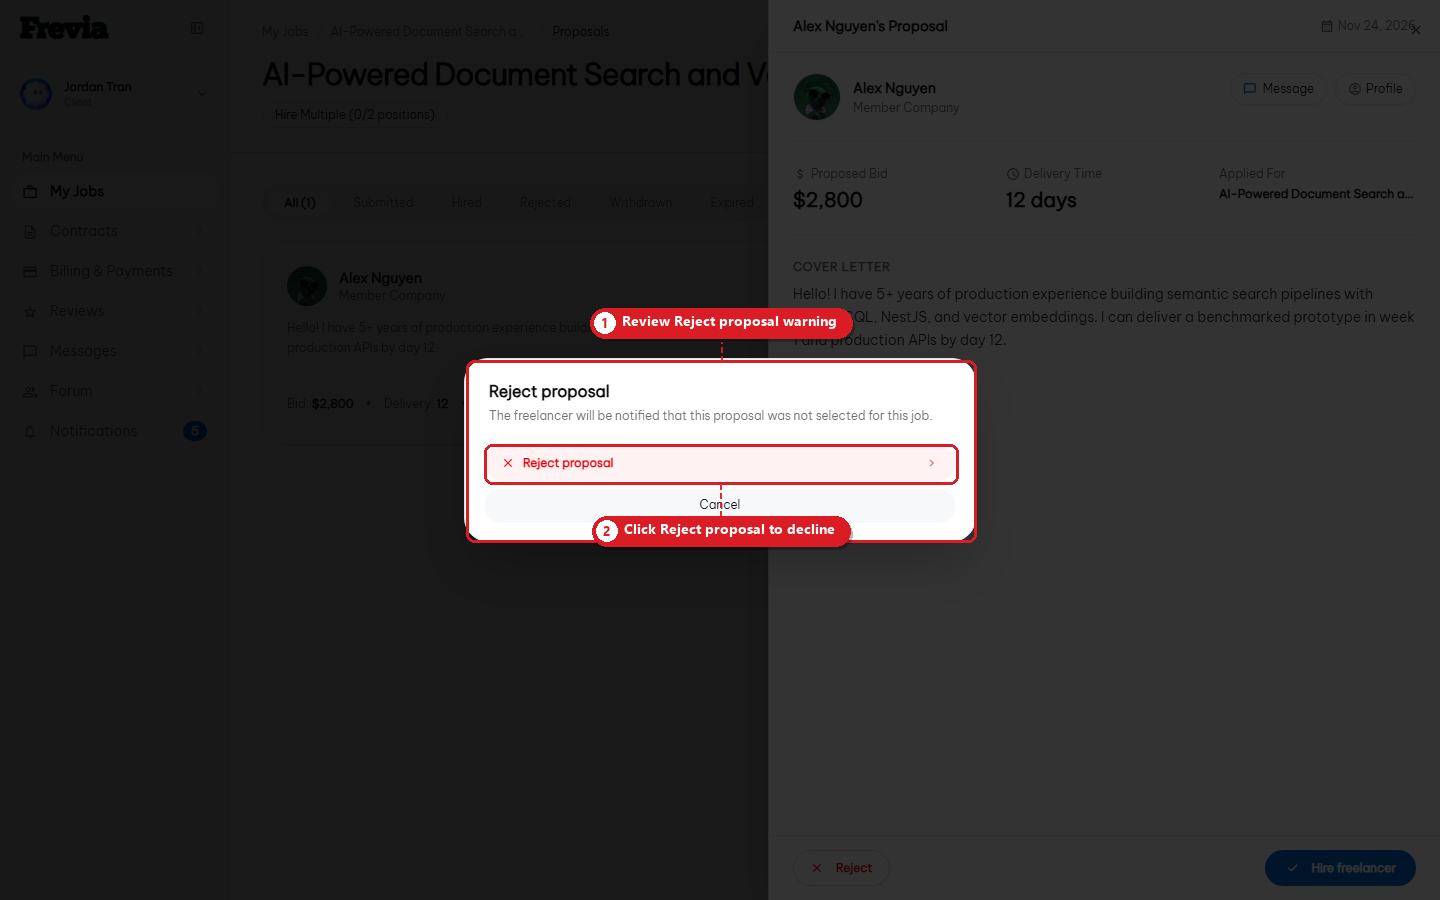
\includegraphics[width=0.90\textwidth]{images/jobs_proposals/m32_07_reject_proposal_guide.png}
  \caption{Reject proposal confirmation modal notifying the Freelancer that their bid was not selected}
  \label{fig:m32_07_reject_proposal}
\end{figure}
\Needspace{6\baselineskip}\paragraph{Step-by-Step User Guide:}
\begin{enumerate}[leftmargin=1.8em,itemsep=3pt]
  \item \rbadge{1} \textbf{Review Decline Notice:} Verify the warning that the Freelancer will be notified that their proposal was not selected.
  \item \rbadge{2} \textbf{Click Reject Proposal:} Click \textbf{Reject proposal} to confirm rejection (or \textbf{Cancel} to keep it under review).
\end{enumerate}
\Needspace{6\baselineskip}\paragraph{After You Submit (Result \& Troubleshooting):}
\begin{itemize}[leftmargin=1.5em,itemsep=2pt]
  \item \textbf{What Happens Next:} Proposal status transitions to \texttt{REJECTED} with a \texttt{rejectedAt} timestamp and moves to the \textbf{Rejected} filter tab.
  \item \textbf{Troubleshooting \& Common Messages:} Only \texttt{SUBMITTED} proposals can be rejected; already hired or withdrawn proposals return HTTP 422 \textit{ProposalNotActionable}.
\end{itemize}

% -----------------------------------------------------------------------------
\newpage
\subsubsection{M32.08 -- View Job Proposals List (UC-34.08)}

\begin{itemize}[leftmargin=1.5em,itemsep=2pt]
  \item \textbf{Screen Name \& Route Path:} Client Job Proposals Pipeline -- \texttt{/client/\allowbreak{}jobs/\allowbreak{}[jobId]/\allowbreak{}proposals}.
  \item \textbf{Target Actor:} Client (Job Owner, Identity Verified).
  \item \Needspace{6\baselineskip}\textbf{Before You Begin:} Open \textbf{My Jobs} (\texttt{/client/jobs}) and click \textbf{View Proposals} on any of your job postings.
\end{itemize}
\begin{figure}[H]\centering
  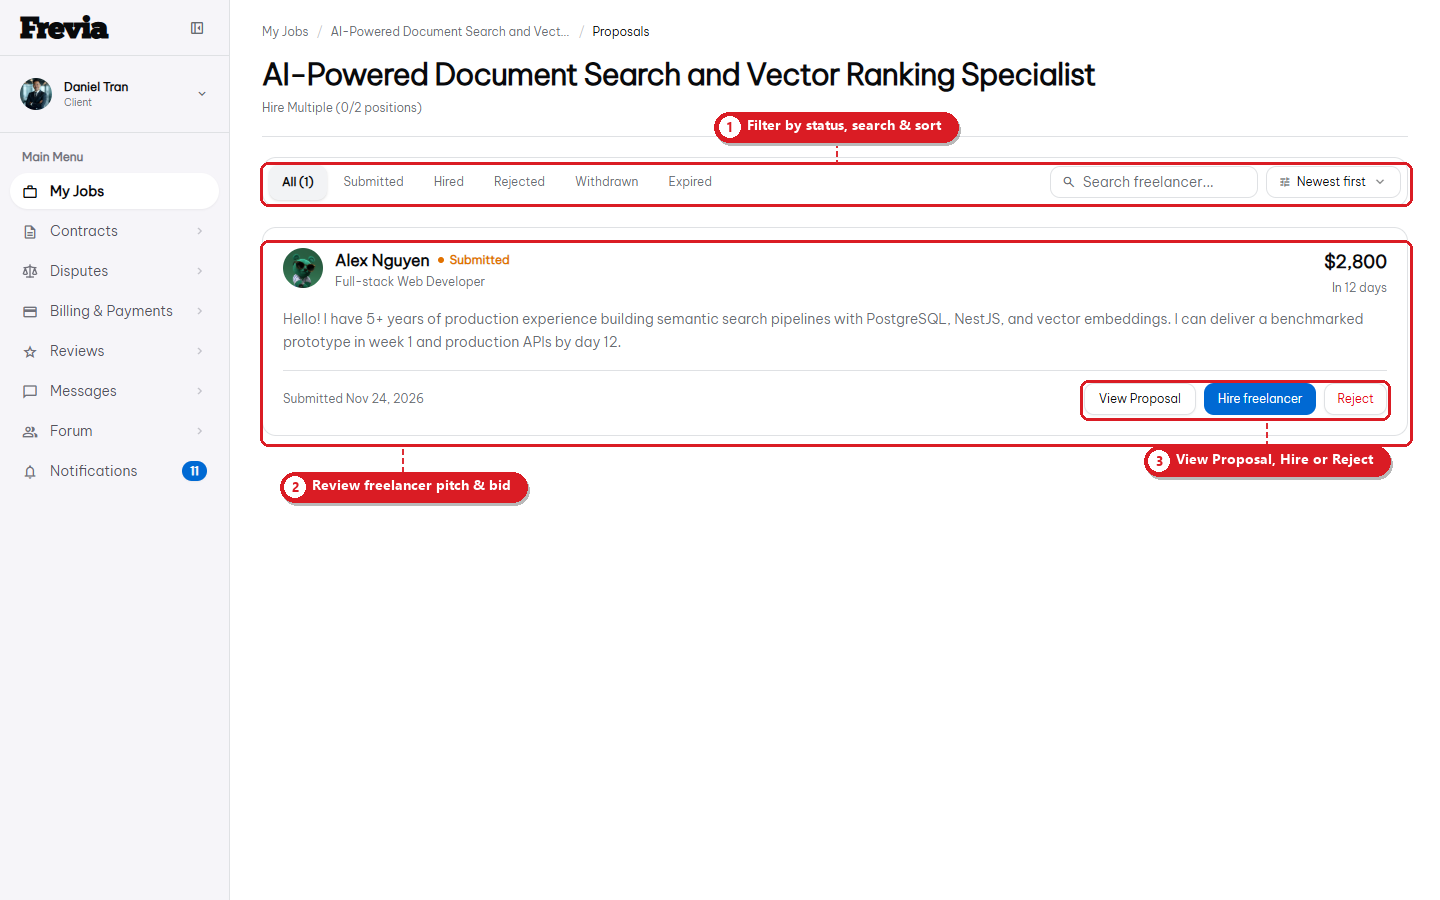
\includegraphics[width=0.90\textwidth]{images/jobs_proposals/m32_08_view_job_proposals_guide.png}
  \caption{Client job proposals pipeline with status filters, freelancer search, sort, and decision buttons}
  \label{fig:m32_08_view_job_proposals}
\end{figure}
\Needspace{6\baselineskip}\paragraph{Step-by-Step User Guide:}
\begin{enumerate}[leftmargin=1.8em,itemsep=3pt]
  \item \rbadge{1} \textbf{Filter, Search \& Sort Applications:} Switch status tabs (\textbf{All}, \textbf{Submitted}, \textbf{Hired}, \textbf{Rejected}, \textbf{Withdrawn}, \textbf{Expired}), search by Freelancer name, or sort by submission date/bid.
  \item \rbadge{2} \textbf{Compare Candidate Cards:} Review each Freelancer's avatar, headline, cover letter excerpt, proposed USD bid, and delivery estimate.
  \item \rbadge{3} \textbf{Take Action:} Click \textbf{View Proposal} to open the detailed drawer, \textbf{Hire freelancer} to accept and draft a contract, or \textbf{Reject} to decline.
\end{enumerate}
\Needspace{6\baselineskip}\paragraph{After You Submit (Result \& Troubleshooting):}
\begin{itemize}[leftmargin=1.5em,itemsep=2pt]
  \item \textbf{What Happens Next:} Overdue proposals are automatically expired before listing; the header badge tracks filled positions (e.g., \textit{Hire Multiple (0/2 positions)}).
  \item \textbf{Troubleshooting \& Common Messages:} Attempting to view proposals for a job owned by another Client returns HTTP 403 \textit{Forbidden}.
\end{itemize}

% -----------------------------------------------------------------------------
\newpage
\subsubsection{M32.09 -- View Proposal Details (Client Drawer) (UC-34.09)}

\begin{itemize}[leftmargin=1.5em,itemsep=2pt]
  \item \textbf{Screen Name \& Route Path:} Proposal Detail Slide-Over Drawer -- \texttt{/client/\allowbreak{}jobs/\allowbreak{}[jobId]/\allowbreak{}proposals}.
  \item \textbf{Target Actor:} Client (Job Owner, Identity Verified).
  \item \Needspace{6\baselineskip}\textbf{Before You Begin:} Click \textbf{View Proposal} on any candidate card in the job proposals pipeline.
\end{itemize}
\begin{figure}[H]\centering
  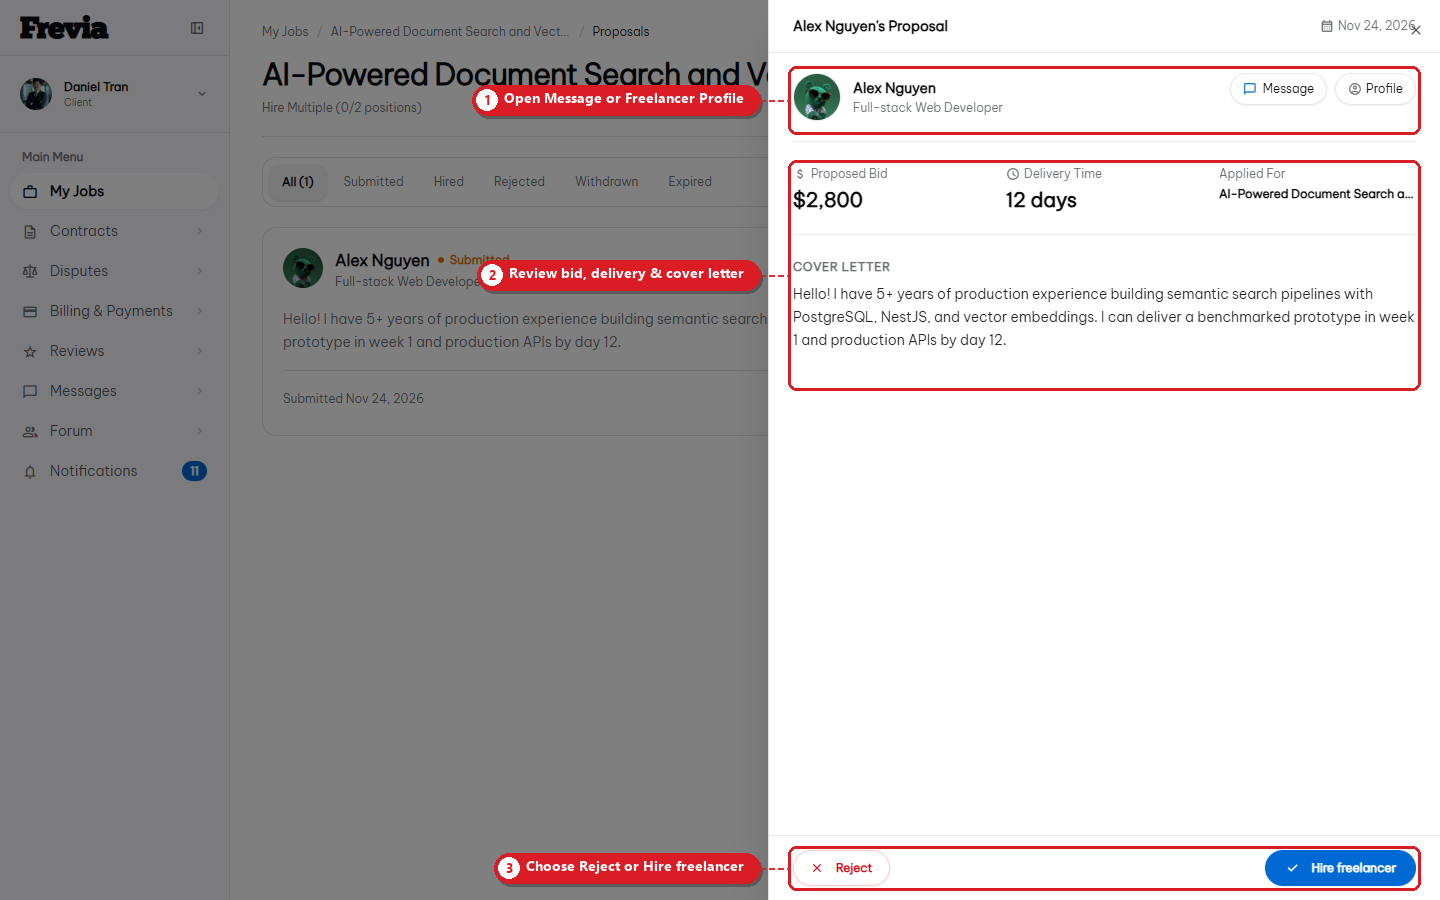
\includegraphics[width=0.90\textwidth]{images/jobs_proposals/m32_09_view_proposal_detail_guide.png}
  \caption{Client Proposal Detail drawer showing candidate shortcuts, bid summary, cover letter, and actions}
  \label{fig:m32_09_view_proposal_detail}
\end{figure}
\Needspace{6\baselineskip}\paragraph{Step-by-Step User Guide:}
\begin{enumerate}[leftmargin=1.8em,itemsep=3pt]
  \item \rbadge{1} \textbf{Message or Inspect Profile:} Click \textbf{Message} to open a direct conversation with the candidate, or click \textbf{Profile} to inspect their full portfolio and verified credentials.
  \item \rbadge{2} \textbf{Read Full Cover Letter \& Terms:} Review the complete \textit{Proposed Bid}, \textit{Delivery Time}, target job title, and full \textit{COVER LETTER}.
  \item \rbadge{3} \textbf{Decide Directly from Drawer:} Click \textbf{Reject} to decline the candidate or \textbf{Hire freelancer} to launch the contract creation sheet.
\end{enumerate}
\Needspace{6\baselineskip}\paragraph{After You Submit (Result \& Troubleshooting):}
\begin{itemize}[leftmargin=1.5em,itemsep=2pt]
  \item \textbf{What Happens Next:} The slide-over keeps your place in the proposal list while letting you inspect and act on candidates quickly.
  \item \textbf{Troubleshooting \& Common Messages:} If the Freelancer withdrew their proposal while the drawer was open, action buttons refresh and display HTTP 422 \textit{ProposalNotActionable}.
\end{itemize}

% -----------------------------------------------------------------------------
\newpage
\subsubsection{M42.01 -- AI Job \& Freelancer Recommendations (UC-44.01)}

\begin{itemize}[leftmargin=1.5em,itemsep=2pt]
  \item \textbf{Screen Name \& Route Path:} Best Matches Recommendation Feed -- \texttt{/freelancer/\allowbreak{}find-work/\allowbreak{}best-matches}; Client Candidate Ranking API -- \texttt{GET /api/\allowbreak{}recommendations/\allowbreak{}freelancers}.
  \item \textbf{Target Actor:} Freelancer, Client, AI Recommendation System.
  \item \Needspace{6\baselineskip}\textbf{Before You Begin:} Complete your Freelancer profile and skills (and optionally upload a PDF CV) for optimal AI matching accuracy.
\end{itemize}
\begin{figure}[H]\centering
  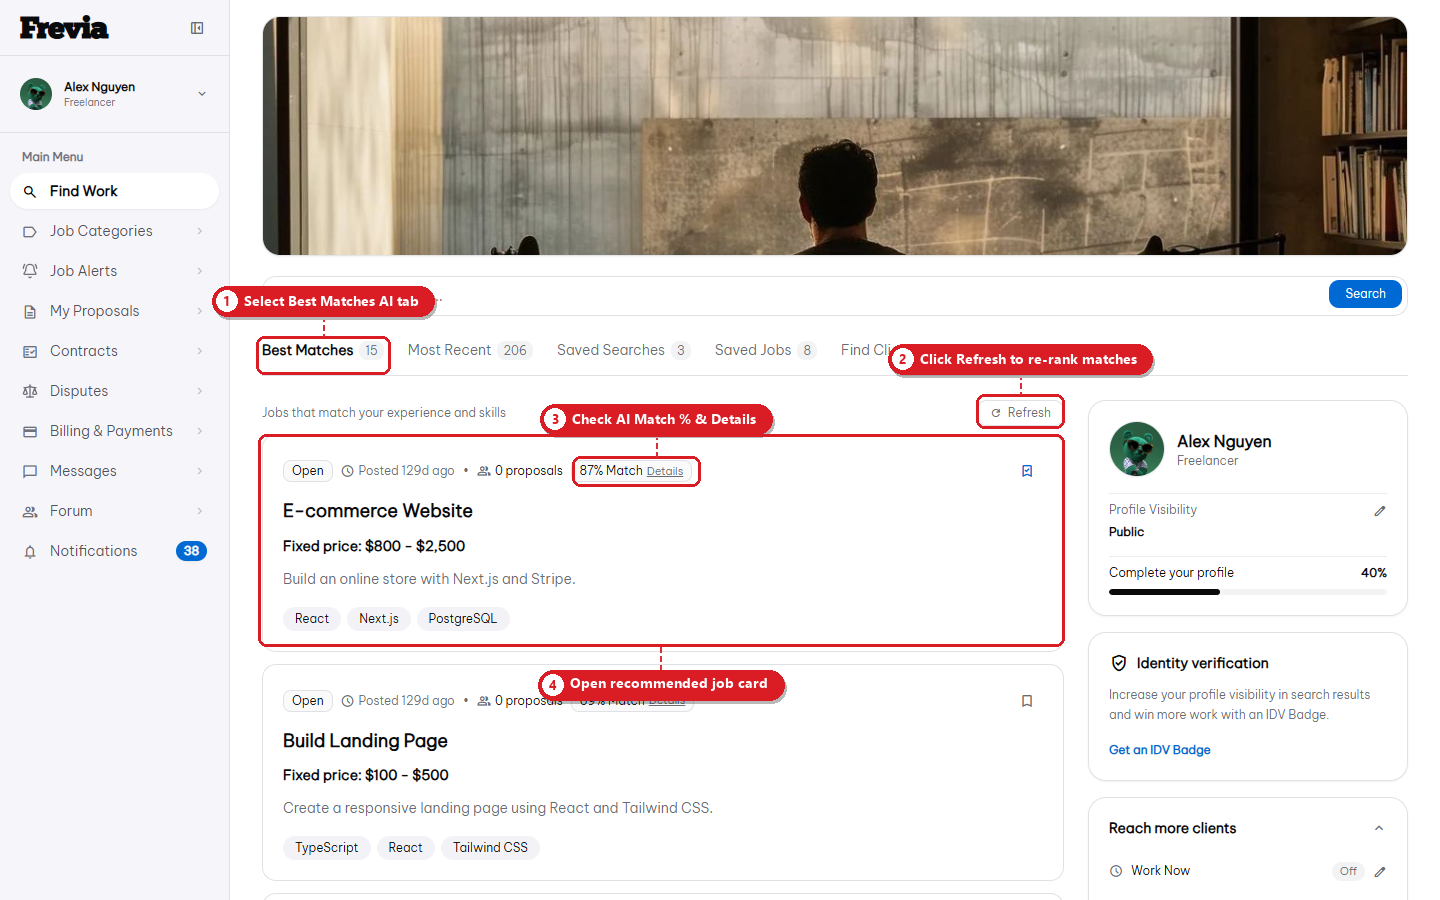
\includegraphics[width=0.90\textwidth]{images/jobs_proposals/m42_01_ai_job_recommendations_guide.png}
  \caption{Freelancer Best Matches feed displaying AI composite match percentages, Details links, and Refresh}
  \label{fig:m42_01_ai_job_recommendations}
\end{figure}
\Needspace{6\baselineskip}\paragraph{Step-by-Step User Guide:}
\begin{enumerate}[leftmargin=1.8em,itemsep=3pt]
  \item \rbadge{1} \textbf{Select Best Matches Tab:} Open \textbf{Find Work} $\rightarrow$ \textbf{Best Matches} to load AI-ranked open job recommendations tailored to your profile and CV (\texttt{cv2jd}).
  \item \rbadge{2} \textbf{Refresh Rankings:} Click \textbf{Refresh} after updating your skills or CV to re-score open jobs via the hybrid \texttt{cv-matching} AI microservice.
  \item \rbadge{3} \textbf{Inspect AI Match Score \& Explanation:} Check the match percentage pill (e.g., \textit{87\% Match}) and click \textbf{Details} to inspect the component score breakdown (semantic, skill, experience, budget, preference) and natural-language AI explanation.
  \item \rbadge{4} \textbf{Open Recommended Job:} Click any recommended job card to inspect full requirements and submit a proposal.
\end{enumerate}
\Needspace{6\baselineskip}\paragraph{After You Submit (Result \& Troubleshooting):}
\begin{itemize}[leftmargin=1.5em,itemsep=2pt]
  \item \textbf{What Happens Next:} Ranked jobs display their live composite match score persisted in PostgreSQL for explanation traceability.
  \item \textbf{Troubleshooting \& Common Messages:} If the AI microservice is temporarily unreachable, the system gracefully falls back to displaying eligible open jobs without blocking browsing; adding more skills to your profile improves score differentiation.
\end{itemize}
